\documentclass[10pt,twocolumn]{article}

% ---- geometry & fonts ----
\usepackage[letterpaper,margin=0.75in]{geometry}
\usepackage[T1]{fontenc}

\usepackage{textcomp}

% ---- maths & graphics ----
\usepackage{amsmath,amssymb,amsfonts}
\usepackage{graphicx}
\usepackage{booktabs}
\usepackage{algorithm}
\usepackage{algpseudocode}
\usepackage{caption}
\usepackage{subcaption}
\usepackage{xcolor}
\usepackage[hidelinks]{hyperref}
\usepackage{cite}

\captionsetup{font=small,labelfont=bf}
\graphicspath{{figures/}}

\setlength{\columnsep}{0.28in}

% ---- title ----
\title{\vspace{-3.5em}\bfseries Spectral Active Learning with Dynamic Model
Management for Uncertainty Quantification of Computationally Expensive
Black-Box Simulators}

\author{%
Vora Yugam Jinesh\\[2pt]
\small Department of Engineering Science, National University of Singapore\\
\small \texttt{https://github.com/Yugam2508/fyp-active-learning-cfd}
}
\date{}

\begin{document}
\maketitle

\begin{abstract}
\noindent
Uncertainty quantification (UQ) for high-fidelity computational fluid
dynamics (CFD) simulations of hazardous gas dispersion is constrained by a
severe budget mismatch: each run costs hours of wall-clock time, while
classical Monte Carlo UQ needs thousands of evaluations. Surrogate models
bridge this gap, but we identify and characterise a specific catastrophic
failure mode of the standard tool---Gaussian Process (GP) regression---under
which it is unsafe to deploy passively. We show experimentally that GP
\emph{prior reversion} produces near-constant, physically meaningless
predictions only when \emph{two} conditions hold simultaneously: a large
input domain relative to the sampling budget, \emph{and} a high
output dynamic range. A domain-size ablation locates a sharp crossover
between half-widths $2$ and $10$, and a Schwefel control
($\rho{=}1.09$) confirms that large domain size alone is insufficient. To
recover performance within the same budget we propose an active learning
framework combining a heterogeneous surrogate committee, a spectral
uncertainty acquisition metric (UEigV) derived from the normalised graph
Laplacian of the committee prediction graph, and a consistency-based model
manager available in a hard-rejection (LCS) and a soft, reversible
cross-validation-weighted variant. On the target regime the framework
reduces RMSE $23$-fold at an equal budget of $20$ evaluations. We then
complete the pipeline with a forward-UQ stage that propagates the input
distribution through the trained committee to deliver an output probability
box, bounded exceedance probabilities, a law-of-total-variance
epistemic/aleatoric decomposition that doubles as a convergence diagnostic,
and Sobol sensitivity indices with epistemic error bars---all validated
against ground-truth Monte Carlo. We give an honest delineation of where the
framework wins and where a passive GP suffices.
\end{abstract}

\section{Introduction}
The transition toward low-carbon energy has renewed interest in ammonia as a
hydrogen carrier, but ammonia is toxic and accidental releases form dense,
ground-hugging clouds whose spatial concentration must be predicted for
quantitative risk assessment~\cite{tan2017}. CFD is the industry standard for
such dispersion modelling, solving the Navier--Stokes equations coupled with
species transport, but a single high-resolution run can take hours to days on
HPC infrastructure. This expense is a fundamental barrier to UQ: Monte Carlo
(MC) converges as $N^{-1/2}$~\cite{jcgm2008}, so reducing error tenfold needs
$100\times$ more runs, while the feasible CFD budget is often fewer than
twenty evaluations.

Surrogate models---cheap emulators trained on a handful of high-fidelity
evaluations---are the standard remedy~\cite{wang2022,heidenreich2017}, with
GP regression the workhorse for computer experiments~\cite{sacks1989,rw2006}.
A surrogate that is overconfident in data-sparse regions, however,
contributes model-form uncertainty invisible to its own variance
estimate~\cite{huellermeier2021}. We make this concrete by characterising
\emph{GP prior reversion}: when the average inter-sample distance exceeds the
learnable kernel length scale, GP predictions collapse to the prior mean. For
high-dynamic-range responses---like CFD concentration fields spanning orders
of magnitude---this prior mean is catastrophically wrong.

This paper makes four contributions. \textbf{(1)} A falsifiable,
two-condition criterion (large domain $\times$ high dynamic range) for when
passive GP surrogates fail catastrophically, supported by a domain-size
ablation and a Schwefel control. \textbf{(2)} A spectral active learning
framework whose acquisition metric, UEigV, transfers the graph-Laplacian
uncertainty measure of~\cite{lin2024} from language-model UQ to physical
surrogate modelling for the first time. \textbf{(3)} A consistency-based
model manager in two forms---hard Largest Consistent Subset (LCS) rejection
and a soft, reversible cross-validation-weighted variant---and an analysis of
why naive soft schemes fail. \textbf{(4)} A forward-UQ stage that turns the
trained committee into a Monte Carlo engine delivering a probability box,
bounded exceedance probabilities, a variance decomposition that serves as a
stopping diagnostic, and Sobol indices with epistemic bars.

\section{Failure Characterisation}
\label{sec:failure}
For a GP with prior mean $\mu$ and kernel $k$, the posterior predictive mean
at a test point $\mathbf{x}^\ast$ is
\begin{equation}
\hat f(\mathbf{x}^\ast)=\mu+\mathbf{k}_\ast^\top
\!\left(\mathbf{K}+\sigma_\varepsilon^2\mathbf{I}\right)^{-1}\!(\mathbf{y}-\mu\mathbf{1}).
\label{eq:gp}
\end{equation}
As the minimum distance between $\mathbf{x}^\ast$ and the training set grows
relative to the length scale $\ell$, the RBF covariance
$k(\mathbf{x}^\ast,\mathbf{x}_i)\!=\!\sigma_f^2\exp(-\lVert\mathbf{x}^\ast-\mathbf{x}_i\rVert^2/2\ell^2)\!\to\!0$,
so $\hat f\to\mu$ regardless of the data. On the physics benchmark
$f_{\text{phys}}(\mathbf{x})=\sin(2x_1)\cos(2x_2)+e^{-x_3^2}+0.2\lVert\mathbf{x}\rVert^2$
over $[-200,200]^3$, with $20$ Latin-Hypercube (LHS) samples the expected
nearest-neighbour distance is $\mathcal{O}(100)$ per dimension; the marginal
likelihood cannot identify a length scale long enough to bridge the gaps, and
the GP reverts to its standardised prior mean across most of the domain.

\paragraph{Domain-size ablation.} Figure~\ref{fig:ablation} evaluates the
benchmark at half-widths $h\in\{2,10,50,100,200\}$ with all other settings
fixed. A sharp crossover appears between $h{=}2$ ($\rho{=}1.06$,
indistinguishable) and $h{=}10$ ($\rho{=}0.384$), where
$\rho=\text{RMSE}_{\text{AL}}/\text{RMSE}_{\text{LHS+GP}}$. The peak advantage
$\rho{=}0.005$ (a $200\times$ reduction) occurs at $h{=}50$.

\paragraph{The Schwefel control.} The Schwefel function on $[-500,500]^3$ has
a \emph{larger} domain than the physics benchmark, yet active learning does
not win ($\rho{=}1.09$). Its output varies only between $\pm 418d$ with the
minimum near zero, so the GP prior mean is a reasonable approximation even in
data-sparse regions. This isolates the mechanism: catastrophic failure
requires large domain size \emph{and} high output dynamic range. This
two-condition criterion is the central empirical finding.

\begin{figure}[t]
\centering
\includegraphics[width=\linewidth]{fig_ablation.pdf}
\caption{Domain-size ablation on the physics benchmark ($30$ trials, $N{=}20$
per method). Left: RMSE ratio $\rho$ versus half-width; the shaded band is the
crossover zone. Right: absolute mean RMSE; the trajectories diverge as the
domain grows.}
\label{fig:ablation}
\end{figure}

\section{Spectral Active Learning Framework}
\label{sec:framework}

\paragraph{Heterogeneous committee.} A committee of up to $K{=}9$ surrogates
spans complementary inductive biases: two GPs (RBF and Mat\'ern-$3/2$), two
Polynomial Chaos Expansions (PCE, degrees $2$ and $3$, Bayesian Ridge),
two Random Forests ($50$/$100$ trees), an RBF Support Vector Regressor, and
two dropout DNNs ($2{\times}64$, $2{\times}128$). Structural heterogeneity is
essential because identical models share a failure mode and reveal no
model-form uncertainty~\cite{lakshmi2017}.

\paragraph{UEigV acquisition.} At a candidate $\mathbf{x}$ the $K$ predictions
form nodes of a fully connected graph with RBF edge weights
$A_{ij}=\exp(-(\hat y_i-\hat y_j)^2/2\sigma^2)$. With normalised Laplacian
$\mathbf{L}=\mathbf{I}-\mathbf{D}^{-1/2}\mathbf{A}\mathbf{D}^{-1/2}$ and
eigenvalues $\lambda_k\in[0,2]$, the acquisition score is
\begin{equation}
\text{UEigV}(\mathbf{x})=\sum_{k=1}^{K}\max\!\left(0,\,1-\lambda_k\right),
\label{eq:ueigv}
\end{equation}
a continuous relaxation of the number of agreement clusters~\cite{lin2024}.
Full consensus gives $\text{UEigV}\approx 0$; a two-way split gives
$\approx 2$. The next query maximises UEigV over a proximity-filtered random
candidate pool. Different families extrapolate differently in data-sparse
regions---a GP reverts to its mean, a PCE follows the global polynomial, an RF
returns leaf means---so UEigV is high precisely where the function is least
constrained.

\paragraph{Model management.} Not all surrogates learn at the same rate;
high-capacity DNNs overfit early and inject phantom disagreement into UEigV.
The \emph{hard} LCS manager scores each model by its reduced chi-square
deviation from the ensemble mean and permanently rejects the worst if it
exceeds the $\alpha$-quantile threshold (with a minimum-data guard and a
floor of two active models). We use the ensemble mean, not the true values,
as the reference: every surrogate interpolates the sparse training data, so
training-point residuals against truth are uninformative; relative
consistency is the criterion that discriminates in the active-learning
regime. We set $\alpha{=}0.99$, identified by sensitivity analysis as the best
diversity--stability balance.

\begin{algorithm}[t]
\caption{Spectral Active Learning with model management}
\label{alg:al}
\begin{algorithmic}[1]
\Require domain $\mathcal{X}$, budget $N_{\max}$, $N_0{=}5$, threshold $\alpha$
\State $\mathcal{D}_0\gets\text{LHS}(N_0,\mathcal{X})$; train committee on $\mathcal{D}_0$
\For{$t=1,\dots,N_{\max}-N_0$}
  \State sample candidate pool $\mathcal{X}_c$ (proximity-filtered)
  \State $\mathbf{x}^\ast\gets\arg\max_{\mathbf{x}\in\mathcal{X}_c}\text{UEigV}(\mathbf{x})$
  \State $y^\ast\gets f(\mathbf{x}^\ast)$;\;\; $\mathcal{D}_t\gets\mathcal{D}_{t-1}\cup\{(\mathbf{x}^\ast,y^\ast)\}$
  \State retrain all active models on $\mathcal{D}_t$
  \State apply model manager (hard LCS \emph{or} soft CV weights)
\EndFor
\State \Return committee, $\mathcal{D}_{N_{\max}}$
\end{algorithmic}
\end{algorithm}

\paragraph{Soft, reversible weighting.} Permanent rejection is irreversible:
a DNN that is useless at $N{=}8$ but informative at $N{=}16$ is gone for good.
We therefore offer a soft variant that weights rather than removes. The
working scheme uses $k$-fold cross-validation error,
\begin{equation}
w_k\;\propto\;\frac{1}{\text{CV-MSE}_k\,(1+\pi_k)},
\label{eq:soft}
\end{equation}
i.e.\ inverse-variance (weighted-average-surrogate) weighting~\cite{goel2007,
viana2009}, with an optional physics penalty $\pi_k\ge0$ for violations of
known output bounds (e.g.\ concentration non-negativity), in the spirit of
physics-informed ML~\cite{karniadakis2021}. Models below a weight floor are
\emph{transiently} muted from the UEigV graph but keep retraining and may
recover. Two natural alternatives \emph{fail} and are instructive: (i)
Boltzmann weights on the training-point chi-square score
($w_k\!\propto\!e^{-s_k/2T}$) leave catastrophic extrapolators near-uniformly
weighted because the score cannot separate models that all interpolate the
data, contaminating the mixture; (ii) consensus-deviation probe scores punish
the single \emph{correct} dissenter when the majority prior-reverts together.
CV error sidesteps both by scoring against held-out data, separating members
by orders of magnitude.

\section{Cross-Benchmark Results}
\label{sec:results}
All methods use a fixed budget of $N{=}20$ ($5$ initial LHS $+$ $15$ steps)
over $30$ independent trials, with RMSE on a $5{,}000$-point held-out set.

\begin{table}[t]
\centering
\caption{Cross-benchmark performance, $N{=}20$, $30$ trials.
$\rho=\overline{\text{RMSE}}_{\text{AL}}/\overline{\text{RMSE}}_{\text{LHS+GP}}$.}
\label{tab:cross}
\small
\begin{tabular}{@{}lrrr@{}}
\toprule
Problem & AL mean & LHS+GP & $\rho$ \\
\midrule
Physics $[-200,200]^3$ & $111$   & $2{,}504$ & $\mathbf{0.044}$ \\
Borehole (8-D)         & $15.06$ & $13.57$   & $1.110$ \\
Piston (7-D)           & $0.105$ & $0.093$   & $1.133$ \\
Friedman (5-D)         & $2.887$ & $2.467$   & $1.170$ \\
Nonstationary (3-D)    & $0.792$ & $0.839$   & $0.944$ \\
Branin (2-D)           & $23.57$ & $20.46$   & $1.152$ \\
Hartmann3 (3-D)        & $0.658$ & $0.570$   & $1.156$ \\
Ishigami (3-D)         & $3.941$ & $3.605$   & $1.093$ \\
Schwefel (3-D)         & $376$   & $344$     & $1.092$ \\
\bottomrule
\end{tabular}
\end{table}

Table~\ref{tab:cross} and Fig.~\ref{fig:cross} delineate the operating regime
honestly. The physics benchmark---the one problem satisfying both failure
conditions---shows a decisive $23\times$ RMSE reduction ($\rho{=}0.044$). The
nonstationary benchmark is marginally favourable ($\rho{=}0.944$); on the
remaining seven problems a well-specified GP ties or wins by $9$--$17\%$. The
framework does \emph{not} claim universal superiority; it claims a precise,
testable criterion for when adaptive sampling is warranted.

\begin{figure}[t]
\centering
\includegraphics[width=\linewidth]{fig_crossbench.pdf}
\caption{RMSE ratio $\rho$ across nine benchmarks ($N{=}20$, $30$ trials).
Below the dashed break-even line, active learning wins. Only the physics
benchmark (green) shows a decisive advantage.}
\label{fig:cross}
\end{figure}

\paragraph{Success mechanism and an honest caveat.} Instrumenting the runs
shows that the manager sequentially removes the misspecified majority and the
surviving ensemble is anchored by PCE-d2---the exact model class for the
dominant quadratic term, which accounts for $>99.9\%$ of the output variance.
The win is therefore best understood as consistency-based \emph{model
selection} (an anchor-model funnel) with UEigV supplying the disagreement
signal that makes the selection identifiable, rather than a single interior
``discovery'' event. The two-condition criterion is thus necessary but not
sufficient: the committee must also contain a surrogate whose hypothesis
class overlaps the response's dominant structure. In a paired $30$-trial
comparison (identical seeds and initial designs), the soft CV-weighted
variant reproduces this behaviour smoothly and reversibly---median RMSE
$0.64$ vs $0.71$ for hard LCS, success rates $87\%$ vs $90\%$, Wilcoxon
signed-rank $p{=}0.096$: statistical parity in accuracy. Notably, only one
failure seed is shared between the two methods, indicating that failures are
driven by the stochastic query trajectory as well as by initial coverage.

\section{Forward Uncertainty Quantification}
\label{sec:uq}
The trained committee is a Monte Carlo engine: a $50{,}000$-point study costs
seconds on the surrogate versus ${\sim}50{,}000$ CFD-hours on the solver. We
propagate the input distribution through all surrogates and report four
quantities, each with epistemic bars from committee disagreement, validated
against a $200{,}000$-point ground-truth MC on the synthetic benchmark.

\paragraph{Output PDF and probability box.}
Figure~\ref{fig:pbox} shows the CDF probability box: at each level $y$ the
committee CDFs span $[F_{\text{low}}(y),F_{\text{up}}(y)]$, a p-box in the
sense of~\cite{ferson1996}. Exceedance probabilities follow as bounded
intervals: for a $95$th-percentile safety threshold, $P(Y>y_c)$ is returned as
an interval that brackets the truth---the statement a risk assessment needs,
rather than a single unjustified point estimate.

\begin{figure}[t]
\centering
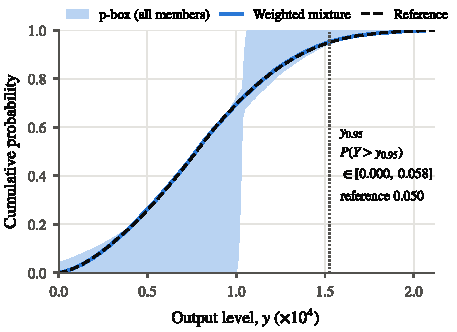
\includegraphics[width=\linewidth]{fig_uq_pbox.pdf}
\caption{CDF probability box and bounded exceedance probability. The band is
the committee envelope, the solid line the weighted-mixture CDF, the dashed
line the ground-truth CDF. The annotated $P(Y>y_c)$ interval brackets truth.}
\label{fig:pbox}
\end{figure}

\paragraph{Variance decomposition as a stopping rule.}
By the law of total variance over the input distribution,
\begin{equation}
\operatorname{Var}[Y]=\underbrace{\operatorname{Var}_{\mathbf{x}}\!\big[\mu_w(\mathbf{x})\big]}_{\text{input-driven}}
+\underbrace{\mathbb{E}_{\mathbf{x}}\!\big[\sigma^2_{\text{epi}}(\mathbf{x})\big]}_{\text{epistemic}}
\;(+\,\sigma^2_\varepsilon).
\label{eq:lotv}
\end{equation}
The epistemic fraction (Fig.~\ref{fig:decomp}) is a convergence diagnostic:
while it dominates, the next evaluation should buy another simulation; once it
is small, the UQ estimate is committee-converged. In our run it decays from
$0.76$ to $\approx 0$ over the budget. This answers the framework's open
problem of online stopping in directly interpretable UQ terms.

\begin{figure}[t]
\centering
\includegraphics[width=\linewidth]{fig_uq_decomp.pdf}
\caption{Law-of-total-variance decomposition versus sample count. Left:
input-driven and epistemic variance. Right: the epistemic fraction, a
convergence/stopping diagnostic.}
\label{fig:decomp}
\end{figure}

\paragraph{Sensitivity with epistemic bars.}
First-order and total Sobol indices are estimated by the Saltelli/Jansen
pick-and-freeze scheme~\cite{saltelli2010,jansen1999} on the cheap ensemble,
with per-model indices furnishing error bars on the sensitivity \emph{ranking}
(Fig.~\ref{fig:sobol}). The ensemble estimates track the ground-truth indices,
closing the loop with classical dispersion sensitivity studies that obtained
the same rankings only by expensive direct MC~\cite{hanna1993}.

\begin{figure}[t]
\centering
\includegraphics[width=\linewidth]{fig_uq_sobol.pdf}
\caption{Sobol first-order and total indices of the weighted ensemble. Error
bars are committee spread (epistemic); black ticks are ground-truth indices.}
\label{fig:sobol}
\end{figure}

Central estimates are accurate for both managers: over $30$ trials the
median relative error of the predicted output median is $0.24\%$ (successful
runs), and a representative run matches truth to within $1\%$ on mean, std,
and all reported quantiles. The managers differ sharply, however, in
\emph{epistemic expressiveness} (Fig.~\ref{fig:campaign}): hard LCS
collapses the committee to a single surviving model in every trial, so its
epistemic bands are degenerate---the mean band and exceedance interval never
cover the truth and the p-box has zero width. The soft variant retains all
nine members with concentrated weights: its mean band covers the true output
mean in $97\%$ of trials and the p-box brackets $57\%$ of the true CDF on
average, though the exceedance interval under-covers in the far upper tail
($13\%$), motivating conformal calibration as future work. Accuracy is at
parity; the capacity to \emph{quantify} model-form uncertainty after
convergence belongs to the soft manager alone.

\begin{figure}[t]
\centering
\includegraphics[width=\linewidth]{fig_campaign.pdf}
\caption{Paired $30$-trial comparison. Left: RMSE distributions (grey lines
join identical seeds); accuracy is at parity. Right: p-box coverage of the
true CDF; hard rejection collapses to one model and loses all epistemic
expressiveness, while soft CV weighting preserves it.}
\label{fig:campaign}
\end{figure}

\section{Discussion and Limitations}
The benchmark is a smooth synthetic construction; real CFD responses include
sharp gradients and recirculation that it does not replicate, so the observed
improvements require validation on a live solver before safety-critical use.
The epistemic bands are committee envelopes, not calibrated probabilities, and
$K{=}9$ gives a coarse envelope---conformal prediction~\cite{angelopoulos2023}
is the principled upgrade. Cross-validation at $N\!\approx\!20$ is itself
noisy, so soft weights should be read as order-of-magnitude statements (which
is all inverse-error weighting needs). Finally, the demonstrated advantage is
partly attributable to PCE-d2 matching the benchmark's dominant term; the
committee must contain a surrogate whose hypothesis class overlaps the true
response. DNN surrogates are two-hidden-layer ReLU networks (Adam,
$800$ epochs, standardised I/O) implemented in PyTorch or, equivalently,
scikit-learn's MLP; the released code supports both backends.

\section{Conclusion}
Passive GP surrogates fail catastrophically precisely when the input domain is
large enough to cause prior reversion \emph{and} the response has high enough
dynamic range to make the prior mean wrong. In that regime, $20$ strategically
selected evaluations achieve a $23\times$ RMSE reduction over $20$ passive
ones via spectral disagreement among structurally diverse surrogates,
stabilised by consistency-based model management---hard or soft. Completed with
a forward-UQ stage delivering a probability box, bounded exceedance
probabilities, a variance-decomposition stopping diagnostic, and Sobol indices
with epistemic bars, the framework provides a principled and honestly
delineated foundation for UQ of expensive black-box simulators, with CFD-based
ammonia dispersion as the motivating application.

\begin{thebibliography}{99}
\small
\bibitem{tan2017} W.\ Tan et al., ``Experimental and numerical study of
ammonia leakage and dispersion in a food factory,'' \emph{J.\ Loss Prev.\
Process Ind.}, vol.\ 47, pp.\ 129--139, 2017.
\bibitem{jcgm2008} JCGM 101:2008, ``Evaluation of measurement data---Supplement
1 to the GUM: Propagation of distributions using a Monte Carlo method,'' 2008.
\bibitem{wang2022} C.\ Wang et al., ``Recent advances in surrogate modeling
methods for UQ and propagation,'' \emph{Symmetry}, vol.\ 14, no.\ 6, 1219,
2022.
\bibitem{heidenreich2017} S.\ Heidenreich et al., ``Uncertainty propagation in
computationally expensive models,'' \emph{Metrologia}, vol.\ 54, pp.\
553--562, 2017.
\bibitem{sacks1989} J.\ Sacks et al., ``Design and analysis of computer
experiments,'' \emph{Statist.\ Sci.}, vol.\ 4, pp.\ 409--423, 1989.
\bibitem{rw2006} C.\ E.\ Rasmussen and C.\ K.\ I.\ Williams, \emph{Gaussian
Processes for Machine Learning}. MIT Press, 2006.
\bibitem{huellermeier2021} E.\ H\"ullermeier and W.\ Waegeman, ``Aleatoric and
epistemic uncertainty in machine learning,'' \emph{Mach.\ Learn.}, vol.\ 110,
pp.\ 457--506, 2021.
\bibitem{lin2024} Z.\ Lin, S.\ Trivedi, and J.\ Sun, ``Generating with
confidence: UQ for black-box LLMs,'' \emph{TMLR}, 2024.
\bibitem{lakshmi2017} B.\ Lakshminarayanan, A.\ Pritzel, and C.\ Blundell,
``Simple and scalable predictive uncertainty estimation using deep
ensembles,'' \emph{NeurIPS}, 2017.
\bibitem{goel2007} T.\ Goel, R.\ T.\ Haftka, W.\ Shyy, and N.\ V.\ Queipo,
``Ensemble of surrogates,'' \emph{Struct.\ Multidiscip.\ Optim.}, vol.\ 33,
pp.\ 199--216, 2007.
\bibitem{viana2009} F.\ A.\ C.\ Viana, R.\ T.\ Haftka, and V.\ Steffen,
``Multiple surrogates: how cross-validation errors can help us to obtain the
best predictor,'' \emph{Struct.\ Multidiscip.\ Optim.}, vol.\ 39, pp.\
439--457, 2009.
\bibitem{karniadakis2021} G.\ E.\ Karniadakis et al., ``Physics-informed
machine learning,'' \emph{Nat.\ Rev.\ Phys.}, vol.\ 3, pp.\ 422--440, 2021.
\bibitem{ferson1996} S.\ Ferson and L.\ R.\ Ginzburg, ``Different methods are
needed to propagate ignorance and variability,'' \emph{Reliab.\ Eng.\ Syst.\
Saf.}, vol.\ 54, pp.\ 133--144, 1996.
\bibitem{saltelli2010} A.\ Saltelli et al., ``Variance based sensitivity
analysis of model output,'' \emph{Comput.\ Phys.\ Commun.}, vol.\ 181, pp.\
259--270, 2010.
\bibitem{jansen1999} M.\ J.\ W.\ Jansen, ``Analysis of variance designs for
model output,'' \emph{Comput.\ Phys.\ Commun.}, vol.\ 117, pp.\ 35--43, 1999.
\bibitem{hanna1993} S.\ R.\ Hanna, D.\ G.\ Strimaitis, and J.\ C.\ Chang,
``Hazard response modeling uncertainty,'' Tech.\ Rep.\ ADA270095, U.S.\ Army
CRDEC, 1993.
\bibitem{angelopoulos2023} A.\ N.\ Angelopoulos and S.\ Bates, ``Conformal
prediction: a gentle introduction,'' \emph{Found.\ Trends Mach.\ Learn.},
2023.
\end{thebibliography}

\end{document}
